\subsection{Silicon photomultipliers}\label{sec:sipms}
A Silicon PhotoMultiplier (SiPM) consists of a matrix of photodiodes (diode which converts light into current), operating in Geiger mode. These photodiodes are connected in parallel becoming each one a pixel of the SiPM. A detailed picture of this structure is shown in figure~\ref{fig:sipm}. The pixels are connected by aluminum stripes to read out the combined signals, which is the sum of all pixels. The pixels are electrically decoupled by polysilicon resistive stripes between the pixels. 

The SiPM used in the NEW detector are the SensL MicroFC-10035-SMT-GP model. This model has demonstrated to be sufficiently radiopure to operate in a low background experiment and also its dark current ($\sim100kHz/mm^2$) is much lower than in the previous models, allowing for easier calibration and an improved threshold for low energy events.


\begin{figure}[h!]
  \centering
  \subfloat[\textit{Detail of the pixel array}]{%\label{fig:cabling:}
  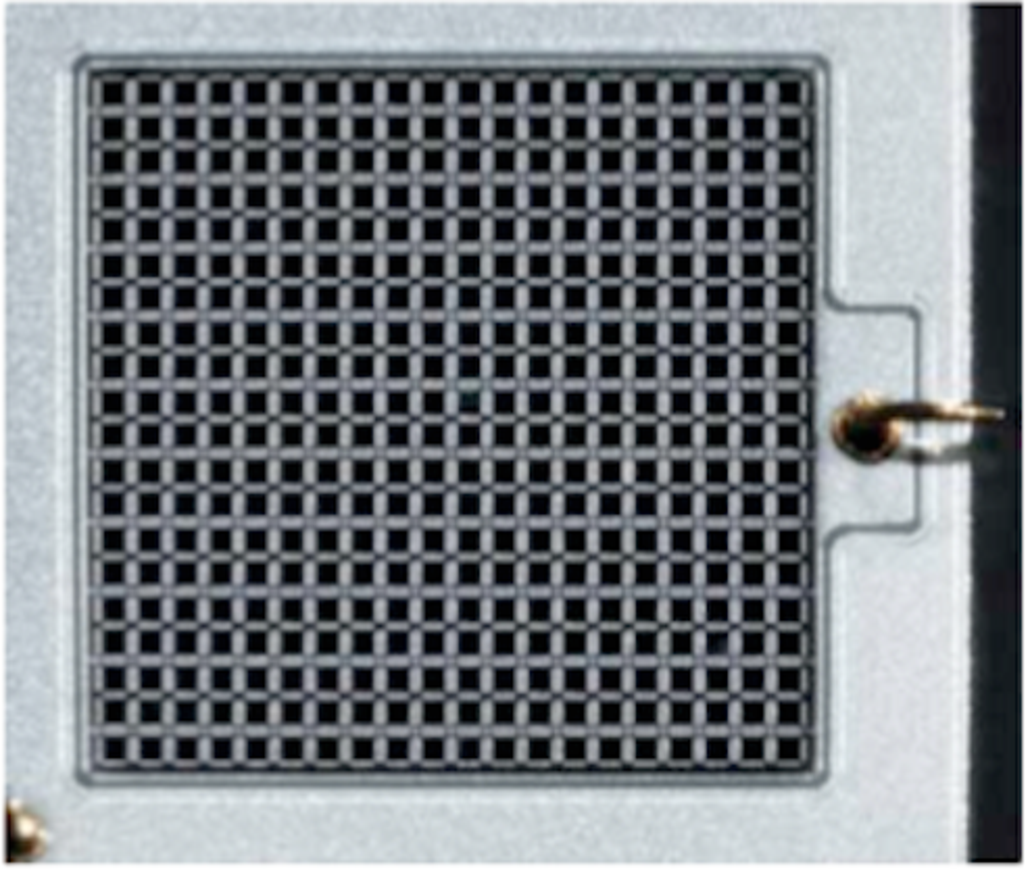
\includegraphics[height=0.22\textwidth]{PixelMatrix.pdf}}   
  \hspace{5mm}             
  \subfloat[\textit{Hamamatsu SiPM}]{%\label{fig:ad:ads7883}
  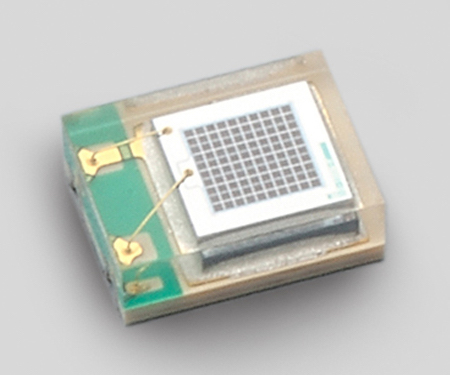
\includegraphics[height=0.22\textwidth]{sipm.jpg}}
  \hspace{5mm}             
  \subfloat[\textit{SiPM from SensL}]{%\label{fig:ad:ads7883}
  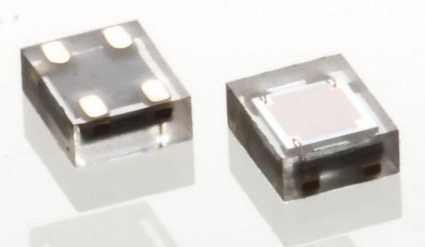
\includegraphics[height=0.22\textwidth]{sensl.jpg}}
  \caption{\textit{Silicon photomultipliers}}
  \label{fig:sipm}
\end{figure}
